\section{Interpolação Parabólica e o Método de Brent}

\vspace{0.5cm}

\subsection{Princípios básicos}

\vspace{0.5cm}

A idéia por trás desse método é utilizar uma aproximação da função $f(x)$ por um polinômio de grau 2 $g(x)$ que passa por três pontos pertencentes a um intervalo enquadrante. Dessa maneira, aproxima-se o mínimo de $f(x)$ pelo mínimo da parábola obtida. A fórmula \ref{eq:parab} permite encontrar a abcissa $x$ correspondente ao mínimo da parábola para os pontos $a,b$ e $c$.\\

\begin{equation}
  x = b - \frac{1}{2}\frac{(b-a)^2[f(b)-f(c)] - (b-c)^2[f(b)-f(a)]}{(b-a)[f(b)-f(c)] - (b-c)[f(b)-f(a)]} 
  \label{eq:parab}
\end{equation}

\vspace{0.5cm}

Redefine-se, então, o intervalo para a próxima iteração de acordo com a avaliação da função objetivo nesses três pontos, descartando o pior deles e guardando o minimizador desta parábola aproximada como novo ponto. Tal interpolação parabólica é dita inversa pois buscamos a abscissa $x$ e não a ordenada $f(x)$. \\

Da expressão \ref{eq:parab}, podemos notar que existe uma singularidade quando os três pontos são colineares. Além disso, o método funciona da mesma maneira tanto na presença de um mínimo quanto de um máximo. \\

Por isso, para contornar tais dificuldades, a estratégia proposta por Brent é utilizar uma busca segura (ex: seção-áurea) quando que a função for não cooperativa e trocar para para interpolação parabólica inversa sempre que possível. Assim, incorpora-se a robustez do método da seção-áurea com a rapidez da interpolação quadrática.\\

\begin{figure}[!h]
\centering
    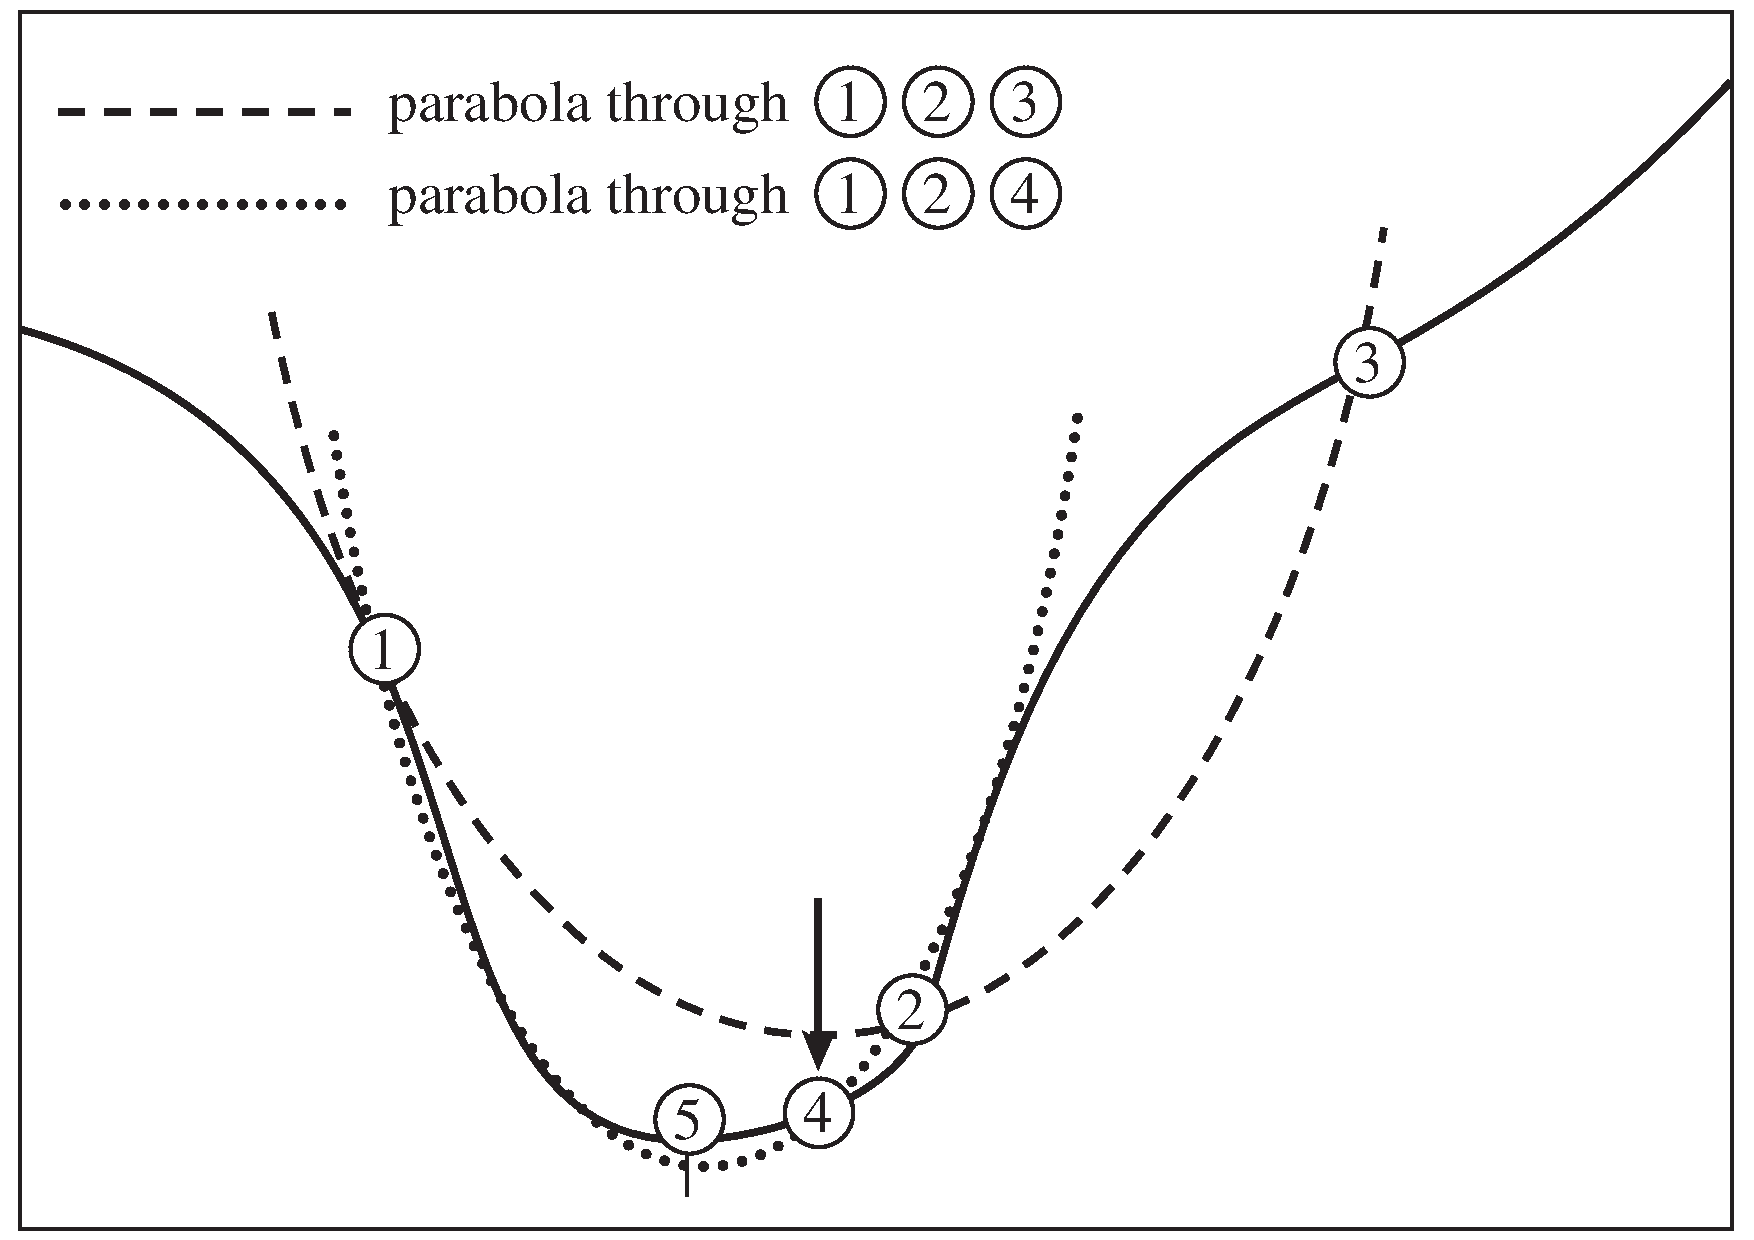
\includegraphics[width=0.75\textwidth]{parabola.pdf}
    \caption{Convergência pelo Método de Brent. Figura retirada de \cite{Brent} }
\label{fig:parabolas}
\end{figure}

A figura \ref{fig:parabolas} mostra duas iterações da interpolação parabólica. É possível notar que a primeira estimativa do minimizador é obtida em $4$ e que, em seguida, esta muda para $5$, se aproximando ainda mais do real valor do minimizador da função $f(x)$.
 
\subsection{Algoritmo}

\vspace{0.5cm}

Durante qualquer fase do algoritmo, este possui um conjunto de 6 pontos $(a, b, u, v, w, x)$. Os pontos $a$ e $b$ definem o intervalo enquadrante de cada iteração; $x$ é o minimizador de $f(x)$ obtido até o momento; $w$ é o ponto de segundo menor valor da função objetivo até o momento e $v$ é o valor anterior de $w$; $u$, por sua vez,  é o ponto onde a função foi avaliada mais recentemente. Um outro ponto que também aparece no algoritmo é o ponto médio entre $a$ e $b$, i.e $x_m$, no entanto, a função objetivo não é avaliada nele.

Se após o passo $d$ da interpolação parabólica, o melhor ponto $x$ pertencer ao intervalo $[a, \, b]$ e, ainda, se o deslocamento provocado por este passo for inferior ao deslocamento provocado na penúltima iteração, significa que $x$ está convergindo e que a interpolação parabólica pode ser usada. Caso alguma dessas condições não seja satisfeita, o passo $d$ é calculado utilizando a razão áurea do maior segmento dentro do intervalo $[a, \,b]$.\\

O algoritmo retoma o início dos cálculos dos novos pontos $(a, b, u, v, w, x)$ até que a tolerância seja atingida ($ |x-x_m| < tol $), alternando,portanto, entre e a interpolação polinomial e o método da razão áurea na determinação dos intervalos para as próximas iterações. O diagrama de fluxo \ref{fig:brentFlow} exemplifica o algoritmo.

 \begin{figure}
 \centering
 \scalebox{1}{% Define block styles
\tikzstyle{io} = [trapezium,trapezium left angle=70,trapezium right angle=-70,minimum height=1cm, draw, fill=yellow!20, text width=6em, text badly centered, node distance=2.5cm, inner sep=0pt]
\tikzstyle{decision} = [diamond, draw, fill=red!20, 
    text width=6em, text badly centered, node distance=3cm, inner sep=0pt]
\tikzstyle{block} = [rectangle, draw, fill=blue!20, 
    text width=10em, text centered, rounded corners, minimum height=4em]
    \tikzstyle{block0} = [rectangle, draw, fill=blue!20, 
    text width=4em, text centered, rounded corners, minimum height=4em]
    \tikzstyle{block1} = [rectangle, draw, fill=cyan!20, node distance=3cm,
    text width=5em, text centered, rounded corners, minimum height=4em]
    \tikzstyle{line} = [draw, -latex']
\tikzstyle{cloud} = [draw, ellipse,fill=green!20, node distance=2cm,
    minimum height=2em]
    \tikzstyle{io2} = [trapezium,trapezium left angle=70,trapezium right angle=-70,minimum height=1cm, draw, fill=yellow!20, text width=1.5cm, text badly centered, node distance=3cm, inner sep=0pt]
    
\begin{tikzpicture}[node distance = 2cm, auto]
    % Place nodes
    \node [io] (input) {$I_1 = [a\, b]$\\$\varepsilon: tolerancia$};
    \node [block, below of =input] (init) {Atualiza $x,w,v,u$\\$x_m = \frac{a+b}{2}$}; % $x=w=v$: criterio 3 pontos\\$d_0=0;
    %\node [block, below of = init] (parab) {Atualiza:\\$x$:minimizador parabola\\$w$:segundo menor valor f\\$v$ : $w$ anterior\\$u$: ultima avaliacao $f$\\};
    \node [block, below of =init] (parab) {$r = (x-w)\,(f_x-f_v)$\\$q = (x-v)\,(f_x-f_w)$\\$p = (x-v)\,q - (x-w)\,r$};
    \node [decision, below of=parab] (evaluate) {$(x+d)\in [a\,b]$\\ $\&\&$\\ $d_k<\frac{d_{k-2}}{2}$};
    \node [below of = evaluate](aux){};
    \node [block1,right of = aux,node distance=3cm] (interp) {$d=\frac{p}{q}$};
    \node [block1, left of=aux, node distance=3cm] (gold) {d: Seção Áurea};
    \node [block0, below of=aux] (act) {$u = x + d$};
    \node [decision, below of=act] (evaluate2) {$|x - x_m|<\varepsilon$};
    \node [io2, below of=evaluate2] (out) {$x_{min}=x$};
    \node [cloud,below of = out] (stop) {FIM};
    %\node [left of = parab_step, node distance=3cm](aux2){};
       
    % Draw edges
    \path [line] (input) -- (init);
    \path [line] (init) -- (parab);
    \path [line] (parab) -- (evaluate);
    \path [line,rounded corners] (evaluate.east) -| node [above] {sim} (interp);
    \path [line,rounded corners] (evaluate.west) -| node [above] {não}(gold);
    \path [line,rounded corners] (gold.south) |- (act.west);
    \path [line,rounded corners] (interp.south) |- (act.east);
    \path[line] (act) -- (evaluate2);
    \path [line] (evaluate2) -- node [near start] {sim} (out);
    \path [line,rounded corners] (evaluate2.east)-- ++(35mm,0mm) |- node [above] {não} (init.east);
    \path [line] (out) -- (stop);
\end{tikzpicture}}
 \caption{Fluxograma do Método de Interpolação}
 \label{fig:brentFlow}
 \end{figure}

\subsection{Resultado}

O resultado obtido para o método de Brent utilizando a função teste apresentada previamente neste relatório (eq. \ref{eq:func_obj}) pode ser observado na figura \ref{fig:brent}.\\

\begin{figure}[h!]
\centering
\scalebox{1}{\section{Interpolação Parabólica e o Método de Brent}

\vspace{0.5cm}

\subsection{Princípios básicos}

\vspace{0.5cm}

A idéia por trás desse método é utilizar uma aproximação da função $f(x)$ por um polinômio de grau 2 $g(x)$ que passa por três pontos pertencentes a um intervalo enquadrante. Dessa maneira, aproxima-se o mínimo de $f(x)$ pelo mínimo da parábola obtida. A fórmula \ref{eq:parab} permite encontrar a abcissa $x$ correspondente ao mínimo da parábola para os pontos $a,b$ e $c$.\\

\begin{equation}
  x = b - \frac{1}{2}\frac{(b-a)^2[f(b)-f(c)] - (b-c)^2[f(b)-f(a)]}{(b-a)[f(b)-f(c)] - (b-c)[f(b)-f(a)]} 
  \label{eq:parab}
\end{equation}

\vspace{0.5cm}

Redefine-se, então, o intervalo para a próxima iteração de acordo com a avaliação da função objetivo nesses três pontos, descartando o pior deles e guardando o minimizador desta parábola aproximada como novo ponto. Tal interpolação parabólica é dita inversa pois buscamos a abscissa $x$ e não a ordenada $f(x)$. \\

Da expressão \ref{eq:parab}, podemos notar que existe uma singularidade quando os três pontos são colineares. Além disso, o método funciona da mesma maneira tanto na presença de um mínimo quanto de um máximo. \\

Por isso, para contornar tais dificuldades, a estratégia proposta por Brent é utilizar uma busca segura (ex: seção-áurea) quando que a função for não cooperativa e trocar para para interpolação parabólica inversa sempre que possível. Assim, incorpora-se a robustez do método da seção-áurea com a rapidez da interpolação quadrática.\\

\begin{figure}[!h]
\centering
    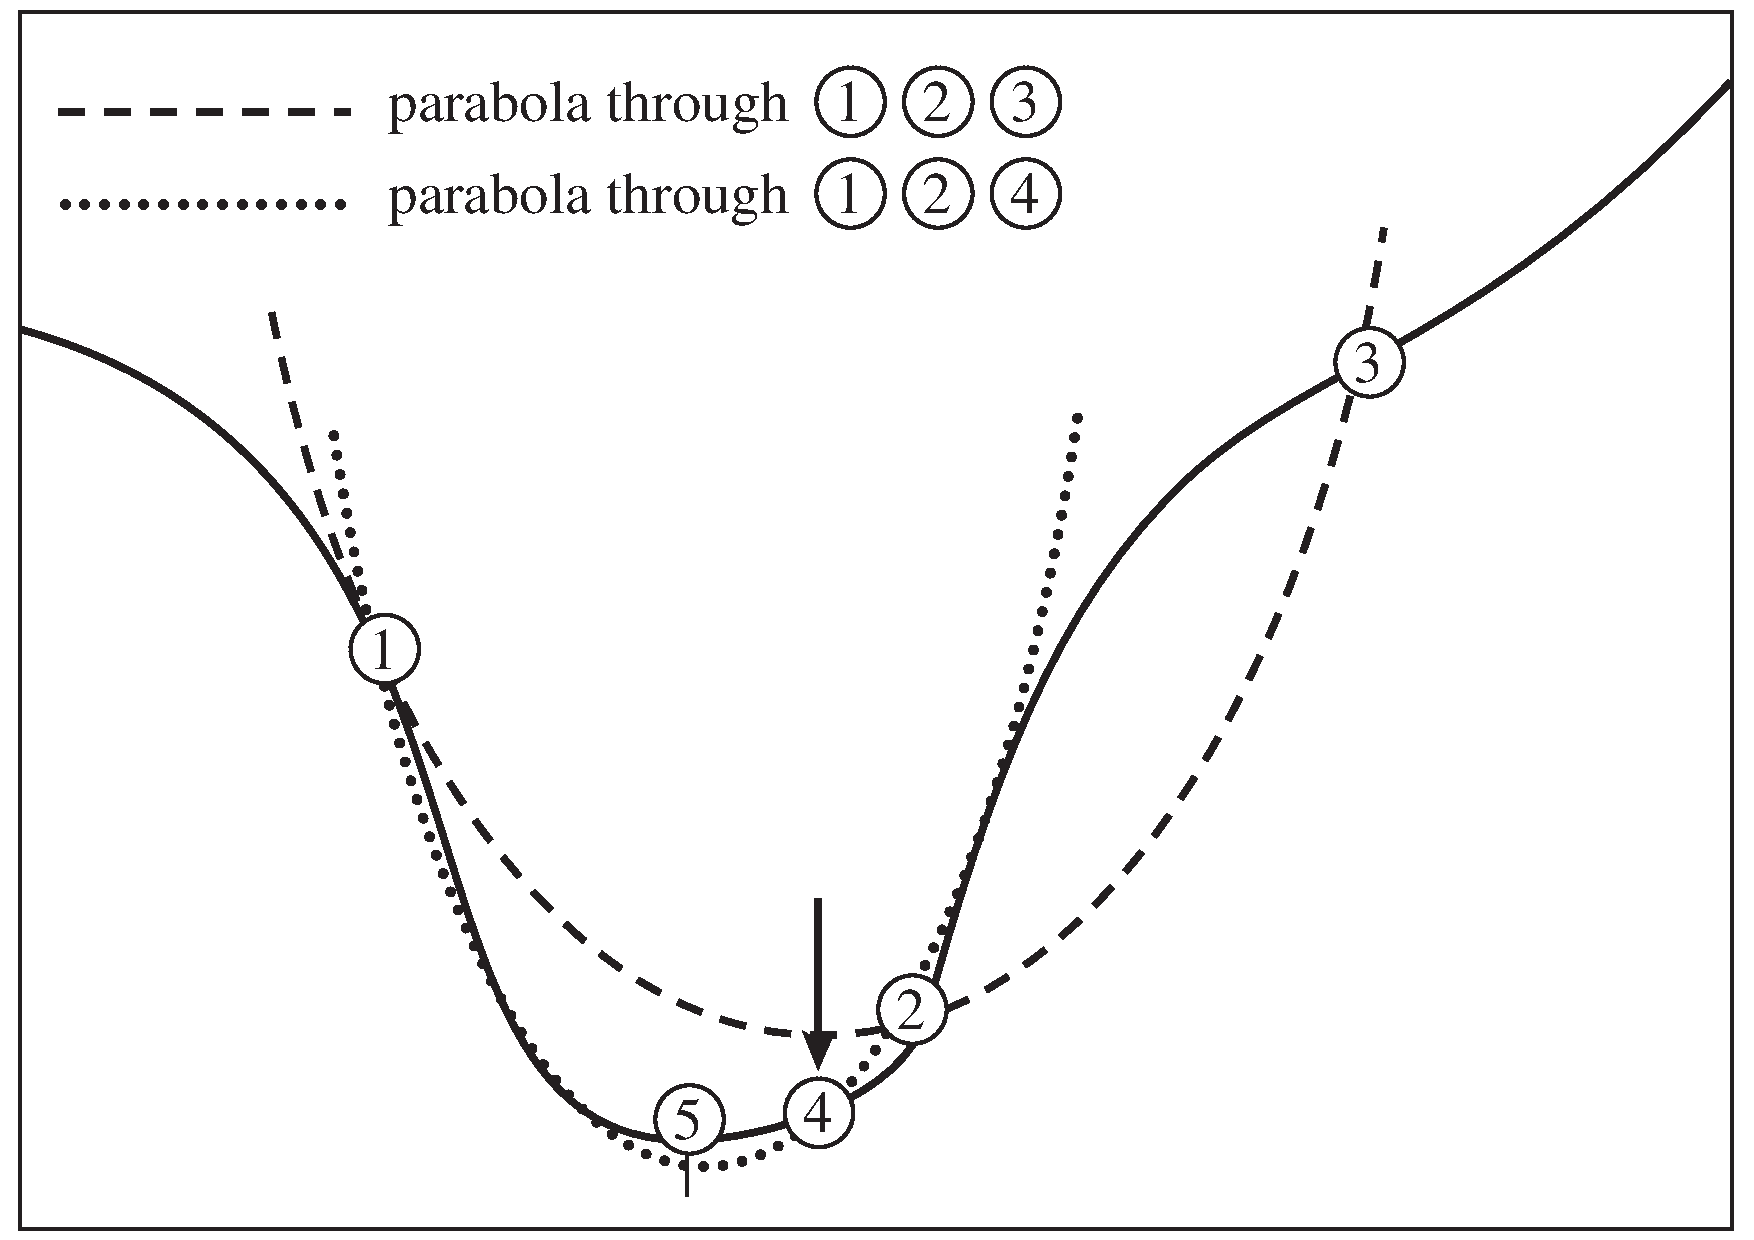
\includegraphics[width=0.75\textwidth]{parabola.pdf}
    \caption{Convergência pelo Método de Brent. Figura retirada de \cite{Brent} }
\label{fig:parabolas}
\end{figure}

A figura \ref{fig:parabolas} mostra duas iterações da interpolação parabólica. É possível notar que a primeira estimativa do minimizador é obtida em $4$ e que, em seguida, esta muda para $5$, se aproximando ainda mais do real valor do minimizador da função $f(x)$.
 
\subsection{Algoritmo}

\vspace{0.5cm}

Durante qualquer fase do algoritmo, este possui um conjunto de 6 pontos $(a, b, u, v, w, x)$. Os pontos $a$ e $b$ definem o intervalo enquadrante de cada iteração; $x$ é o minimizador de $f(x)$ obtido até o momento; $w$ é o ponto de segundo menor valor da função objetivo até o momento e $v$ é o valor anterior de $w$; $u$, por sua vez,  é o ponto onde a função foi avaliada mais recentemente. Um outro ponto que também aparece no algoritmo é o ponto médio entre $a$ e $b$, i.e $x_m$, no entanto, a função objetivo não é avaliada nele.

Se após o passo $d$ da interpolação parabólica, o melhor ponto $x$ pertencer ao intervalo $[a, \, b]$ e, ainda, se o deslocamento provocado por este passo for inferior ao deslocamento provocado na penúltima iteração, significa que $x$ está convergindo e que a interpolação parabólica pode ser usada. Caso alguma dessas condições não seja satisfeita, o passo $d$ é calculado utilizando a razão áurea do maior segmento dentro do intervalo $[a, \,b]$.\\

O algoritmo retoma o início dos cálculos dos novos pontos $(a, b, u, v, w, x)$ até que a tolerância seja atingida ($ |x-x_m| < tol $), alternando,portanto, entre e a interpolação polinomial e o método da razão áurea na determinação dos intervalos para as próximas iterações. O diagrama de fluxo \ref{fig:brentFlow} exemplifica o algoritmo.

 \begin{figure}
 \centering
 \scalebox{1}{% Define block styles
\tikzstyle{io} = [trapezium,trapezium left angle=70,trapezium right angle=-70,minimum height=1cm, draw, fill=yellow!20, text width=6em, text badly centered, node distance=2.5cm, inner sep=0pt]
\tikzstyle{decision} = [diamond, draw, fill=red!20, 
    text width=6em, text badly centered, node distance=3cm, inner sep=0pt]
\tikzstyle{block} = [rectangle, draw, fill=blue!20, 
    text width=10em, text centered, rounded corners, minimum height=4em]
    \tikzstyle{block0} = [rectangle, draw, fill=blue!20, 
    text width=4em, text centered, rounded corners, minimum height=4em]
    \tikzstyle{block1} = [rectangle, draw, fill=cyan!20, node distance=3cm,
    text width=5em, text centered, rounded corners, minimum height=4em]
    \tikzstyle{line} = [draw, -latex']
\tikzstyle{cloud} = [draw, ellipse,fill=green!20, node distance=2cm,
    minimum height=2em]
    \tikzstyle{io2} = [trapezium,trapezium left angle=70,trapezium right angle=-70,minimum height=1cm, draw, fill=yellow!20, text width=1.5cm, text badly centered, node distance=3cm, inner sep=0pt]
    
\begin{tikzpicture}[node distance = 2cm, auto]
    % Place nodes
    \node [io] (input) {$I_1 = [a\, b]$\\$\varepsilon: tolerancia$};
    \node [block, below of =input] (init) {Atualiza $x,w,v,u$\\$x_m = \frac{a+b}{2}$}; % $x=w=v$: criterio 3 pontos\\$d_0=0;
    %\node [block, below of = init] (parab) {Atualiza:\\$x$:minimizador parabola\\$w$:segundo menor valor f\\$v$ : $w$ anterior\\$u$: ultima avaliacao $f$\\};
    \node [block, below of =init] (parab) {$r = (x-w)\,(f_x-f_v)$\\$q = (x-v)\,(f_x-f_w)$\\$p = (x-v)\,q - (x-w)\,r$};
    \node [decision, below of=parab] (evaluate) {$(x+d)\in [a\,b]$\\ $\&\&$\\ $d_k<\frac{d_{k-2}}{2}$};
    \node [below of = evaluate](aux){};
    \node [block1,right of = aux,node distance=3cm] (interp) {$d=\frac{p}{q}$};
    \node [block1, left of=aux, node distance=3cm] (gold) {d: Seção Áurea};
    \node [block0, below of=aux] (act) {$u = x + d$};
    \node [decision, below of=act] (evaluate2) {$|x - x_m|<\varepsilon$};
    \node [io2, below of=evaluate2] (out) {$x_{min}=x$};
    \node [cloud,below of = out] (stop) {FIM};
    %\node [left of = parab_step, node distance=3cm](aux2){};
       
    % Draw edges
    \path [line] (input) -- (init);
    \path [line] (init) -- (parab);
    \path [line] (parab) -- (evaluate);
    \path [line,rounded corners] (evaluate.east) -| node [above] {sim} (interp);
    \path [line,rounded corners] (evaluate.west) -| node [above] {não}(gold);
    \path [line,rounded corners] (gold.south) |- (act.west);
    \path [line,rounded corners] (interp.south) |- (act.east);
    \path[line] (act) -- (evaluate2);
    \path [line] (evaluate2) -- node [near start] {sim} (out);
    \path [line,rounded corners] (evaluate2.east)-- ++(35mm,0mm) |- node [above] {não} (init.east);
    \path [line] (out) -- (stop);
\end{tikzpicture}}
 \caption{Fluxograma do Método de Interpolação}
 \label{fig:brentFlow}
 \end{figure}

\subsection{Resultado}

O resultado obtido para o método de Brent utilizando a função teste apresentada previamente neste relatório (eq. \ref{eq:func_obj}) pode ser observado na figura \ref{fig:brent}.\\

\begin{figure}[h!]
\centering
\scalebox{1}{\section{Interpolação Parabólica e o Método de Brent}

\vspace{0.5cm}

\subsection{Princípios básicos}

\vspace{0.5cm}

A idéia por trás desse método é utilizar uma aproximação da função $f(x)$ por um polinômio de grau 2 $g(x)$ que passa por três pontos pertencentes a um intervalo enquadrante. Dessa maneira, aproxima-se o mínimo de $f(x)$ pelo mínimo da parábola obtida. A fórmula \ref{eq:parab} permite encontrar a abcissa $x$ correspondente ao mínimo da parábola para os pontos $a,b$ e $c$.\\

\begin{equation}
  x = b - \frac{1}{2}\frac{(b-a)^2[f(b)-f(c)] - (b-c)^2[f(b)-f(a)]}{(b-a)[f(b)-f(c)] - (b-c)[f(b)-f(a)]} 
  \label{eq:parab}
\end{equation}

\vspace{0.5cm}

Redefine-se, então, o intervalo para a próxima iteração de acordo com a avaliação da função objetivo nesses três pontos, descartando o pior deles e guardando o minimizador desta parábola aproximada como novo ponto. Tal interpolação parabólica é dita inversa pois buscamos a abscissa $x$ e não a ordenada $f(x)$. \\

Da expressão \ref{eq:parab}, podemos notar que existe uma singularidade quando os três pontos são colineares. Além disso, o método funciona da mesma maneira tanto na presença de um mínimo quanto de um máximo. \\

Por isso, para contornar tais dificuldades, a estratégia proposta por Brent é utilizar uma busca segura (ex: seção-áurea) quando que a função for não cooperativa e trocar para para interpolação parabólica inversa sempre que possível. Assim, incorpora-se a robustez do método da seção-áurea com a rapidez da interpolação quadrática.\\

\begin{figure}[!h]
\centering
    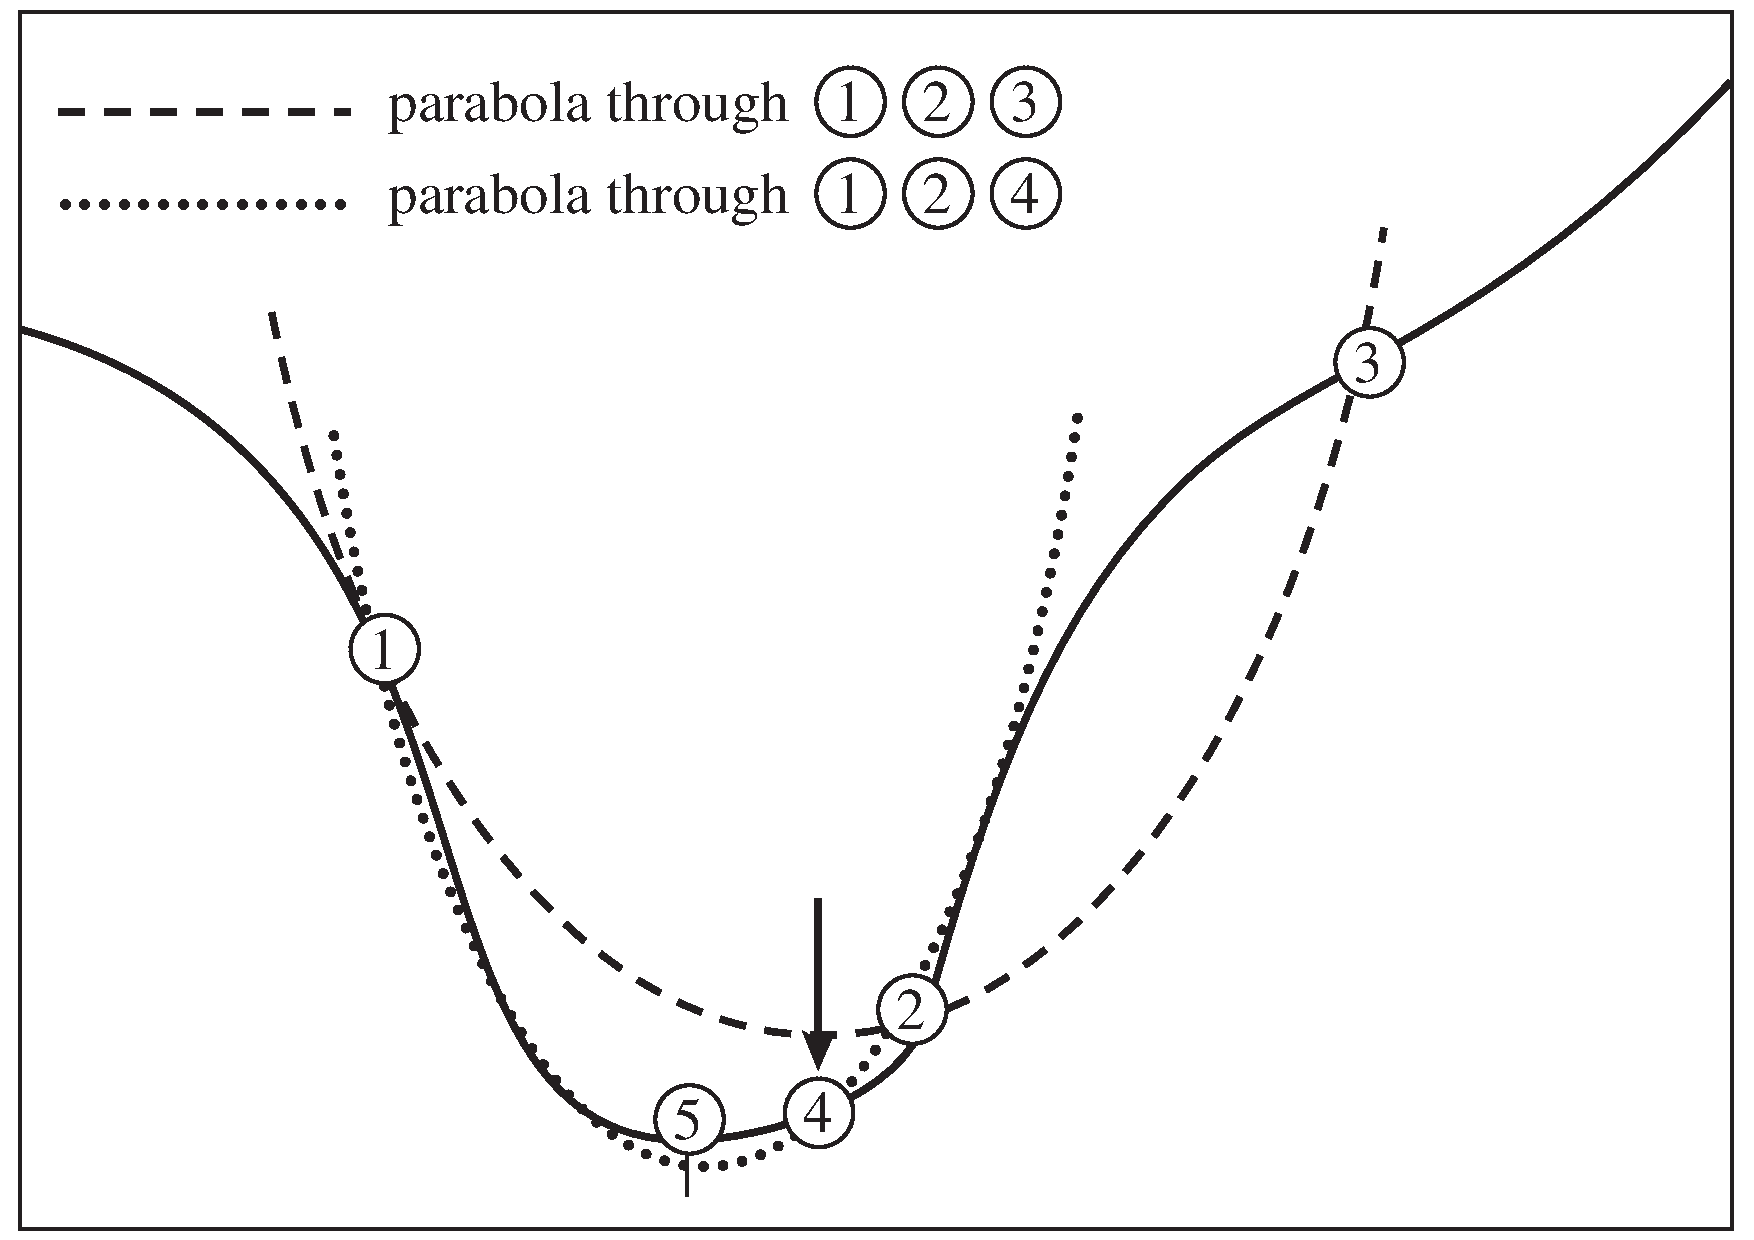
\includegraphics[width=0.75\textwidth]{parabola.pdf}
    \caption{Convergência pelo Método de Brent. Figura retirada de \cite{Brent} }
\label{fig:parabolas}
\end{figure}

A figura \ref{fig:parabolas} mostra duas iterações da interpolação parabólica. É possível notar que a primeira estimativa do minimizador é obtida em $4$ e que, em seguida, esta muda para $5$, se aproximando ainda mais do real valor do minimizador da função $f(x)$.
 
\subsection{Algoritmo}

\vspace{0.5cm}

Durante qualquer fase do algoritmo, este possui um conjunto de 6 pontos $(a, b, u, v, w, x)$. Os pontos $a$ e $b$ definem o intervalo enquadrante de cada iteração; $x$ é o minimizador de $f(x)$ obtido até o momento; $w$ é o ponto de segundo menor valor da função objetivo até o momento e $v$ é o valor anterior de $w$; $u$, por sua vez,  é o ponto onde a função foi avaliada mais recentemente. Um outro ponto que também aparece no algoritmo é o ponto médio entre $a$ e $b$, i.e $x_m$, no entanto, a função objetivo não é avaliada nele.

Se após o passo $d$ da interpolação parabólica, o melhor ponto $x$ pertencer ao intervalo $[a, \, b]$ e, ainda, se o deslocamento provocado por este passo for inferior ao deslocamento provocado na penúltima iteração, significa que $x$ está convergindo e que a interpolação parabólica pode ser usada. Caso alguma dessas condições não seja satisfeita, o passo $d$ é calculado utilizando a razão áurea do maior segmento dentro do intervalo $[a, \,b]$.\\

O algoritmo retoma o início dos cálculos dos novos pontos $(a, b, u, v, w, x)$ até que a tolerância seja atingida ($ |x-x_m| < tol $), alternando,portanto, entre e a interpolação polinomial e o método da razão áurea na determinação dos intervalos para as próximas iterações. O diagrama de fluxo \ref{fig:brentFlow} exemplifica o algoritmo.

 \begin{figure}
 \centering
 \scalebox{1}{% Define block styles
\tikzstyle{io} = [trapezium,trapezium left angle=70,trapezium right angle=-70,minimum height=1cm, draw, fill=yellow!20, text width=6em, text badly centered, node distance=2.5cm, inner sep=0pt]
\tikzstyle{decision} = [diamond, draw, fill=red!20, 
    text width=6em, text badly centered, node distance=3cm, inner sep=0pt]
\tikzstyle{block} = [rectangle, draw, fill=blue!20, 
    text width=10em, text centered, rounded corners, minimum height=4em]
    \tikzstyle{block0} = [rectangle, draw, fill=blue!20, 
    text width=4em, text centered, rounded corners, minimum height=4em]
    \tikzstyle{block1} = [rectangle, draw, fill=cyan!20, node distance=3cm,
    text width=5em, text centered, rounded corners, minimum height=4em]
    \tikzstyle{line} = [draw, -latex']
\tikzstyle{cloud} = [draw, ellipse,fill=green!20, node distance=2cm,
    minimum height=2em]
    \tikzstyle{io2} = [trapezium,trapezium left angle=70,trapezium right angle=-70,minimum height=1cm, draw, fill=yellow!20, text width=1.5cm, text badly centered, node distance=3cm, inner sep=0pt]
    
\begin{tikzpicture}[node distance = 2cm, auto]
    % Place nodes
    \node [io] (input) {$I_1 = [a\, b]$\\$\varepsilon: tolerancia$};
    \node [block, below of =input] (init) {Atualiza $x,w,v,u$\\$x_m = \frac{a+b}{2}$}; % $x=w=v$: criterio 3 pontos\\$d_0=0;
    %\node [block, below of = init] (parab) {Atualiza:\\$x$:minimizador parabola\\$w$:segundo menor valor f\\$v$ : $w$ anterior\\$u$: ultima avaliacao $f$\\};
    \node [block, below of =init] (parab) {$r = (x-w)\,(f_x-f_v)$\\$q = (x-v)\,(f_x-f_w)$\\$p = (x-v)\,q - (x-w)\,r$};
    \node [decision, below of=parab] (evaluate) {$(x+d)\in [a\,b]$\\ $\&\&$\\ $d_k<\frac{d_{k-2}}{2}$};
    \node [below of = evaluate](aux){};
    \node [block1,right of = aux,node distance=3cm] (interp) {$d=\frac{p}{q}$};
    \node [block1, left of=aux, node distance=3cm] (gold) {d: Seção Áurea};
    \node [block0, below of=aux] (act) {$u = x + d$};
    \node [decision, below of=act] (evaluate2) {$|x - x_m|<\varepsilon$};
    \node [io2, below of=evaluate2] (out) {$x_{min}=x$};
    \node [cloud,below of = out] (stop) {FIM};
    %\node [left of = parab_step, node distance=3cm](aux2){};
       
    % Draw edges
    \path [line] (input) -- (init);
    \path [line] (init) -- (parab);
    \path [line] (parab) -- (evaluate);
    \path [line,rounded corners] (evaluate.east) -| node [above] {sim} (interp);
    \path [line,rounded corners] (evaluate.west) -| node [above] {não}(gold);
    \path [line,rounded corners] (gold.south) |- (act.west);
    \path [line,rounded corners] (interp.south) |- (act.east);
    \path[line] (act) -- (evaluate2);
    \path [line] (evaluate2) -- node [near start] {sim} (out);
    \path [line,rounded corners] (evaluate2.east)-- ++(35mm,0mm) |- node [above] {não} (init.east);
    \path [line] (out) -- (stop);
\end{tikzpicture}}
 \caption{Fluxograma do Método de Interpolação}
 \label{fig:brentFlow}
 \end{figure}

\subsection{Resultado}

O resultado obtido para o método de Brent utilizando a função teste apresentada previamente neste relatório (eq. \ref{eq:func_obj}) pode ser observado na figura \ref{fig:brent}.\\

\begin{figure}[h!]
\centering
\scalebox{1}{\section{Interpolação Parabólica e o Método de Brent}

\vspace{0.5cm}

\subsection{Princípios básicos}

\vspace{0.5cm}

A idéia por trás desse método é utilizar uma aproximação da função $f(x)$ por um polinômio de grau 2 $g(x)$ que passa por três pontos pertencentes a um intervalo enquadrante. Dessa maneira, aproxima-se o mínimo de $f(x)$ pelo mínimo da parábola obtida. A fórmula \ref{eq:parab} permite encontrar a abcissa $x$ correspondente ao mínimo da parábola para os pontos $a,b$ e $c$.\\

\begin{equation}
  x = b - \frac{1}{2}\frac{(b-a)^2[f(b)-f(c)] - (b-c)^2[f(b)-f(a)]}{(b-a)[f(b)-f(c)] - (b-c)[f(b)-f(a)]} 
  \label{eq:parab}
\end{equation}

\vspace{0.5cm}

Redefine-se, então, o intervalo para a próxima iteração de acordo com a avaliação da função objetivo nesses três pontos, descartando o pior deles e guardando o minimizador desta parábola aproximada como novo ponto. Tal interpolação parabólica é dita inversa pois buscamos a abscissa $x$ e não a ordenada $f(x)$. \\

Da expressão \ref{eq:parab}, podemos notar que existe uma singularidade quando os três pontos são colineares. Além disso, o método funciona da mesma maneira tanto na presença de um mínimo quanto de um máximo. \\

Por isso, para contornar tais dificuldades, a estratégia proposta por Brent é utilizar uma busca segura (ex: seção-áurea) quando que a função for não cooperativa e trocar para para interpolação parabólica inversa sempre que possível. Assim, incorpora-se a robustez do método da seção-áurea com a rapidez da interpolação quadrática.\\

\begin{figure}[!h]
\centering
    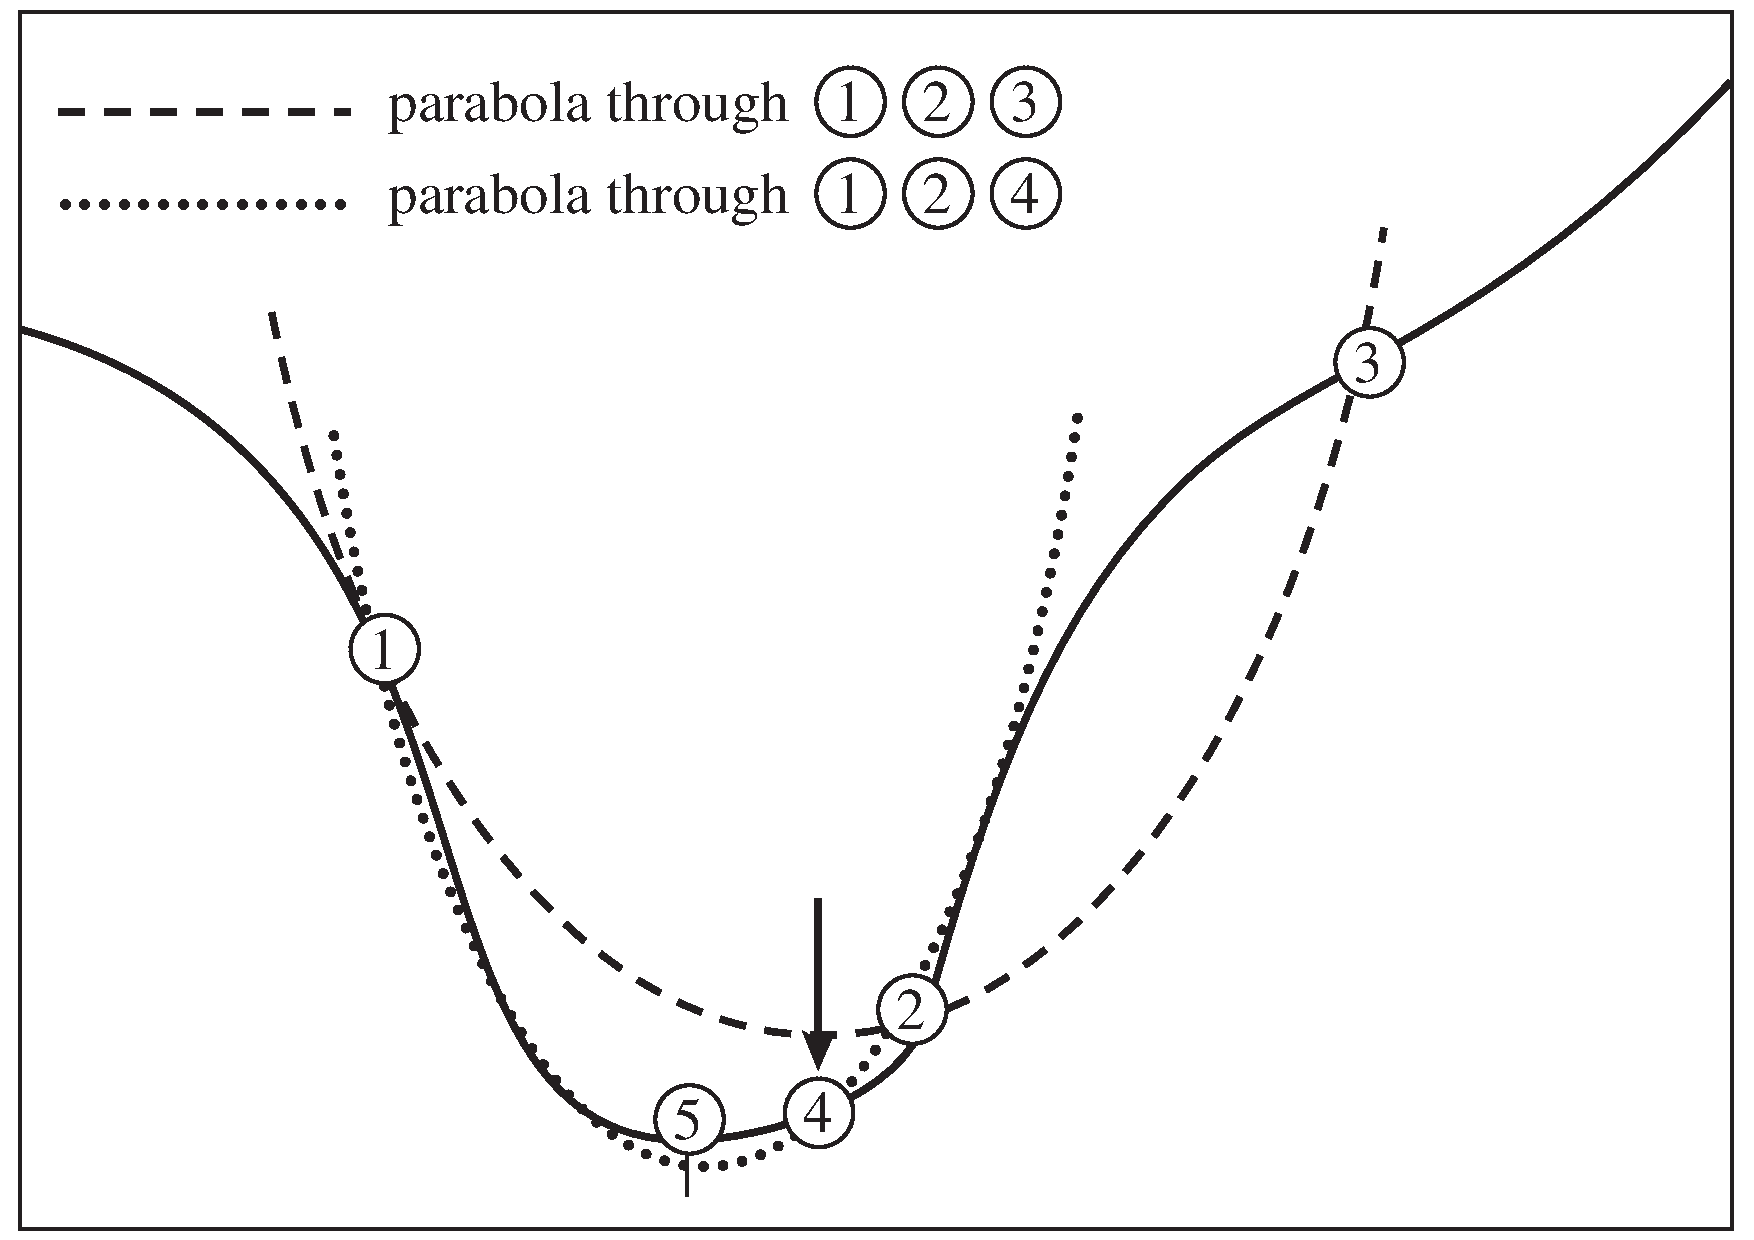
\includegraphics[width=0.75\textwidth]{parabola.pdf}
    \caption{Convergência pelo Método de Brent. Figura retirada de \cite{Brent} }
\label{fig:parabolas}
\end{figure}

A figura \ref{fig:parabolas} mostra duas iterações da interpolação parabólica. É possível notar que a primeira estimativa do minimizador é obtida em $4$ e que, em seguida, esta muda para $5$, se aproximando ainda mais do real valor do minimizador da função $f(x)$.
 
\subsection{Algoritmo}

\vspace{0.5cm}

Durante qualquer fase do algoritmo, este possui um conjunto de 6 pontos $(a, b, u, v, w, x)$. Os pontos $a$ e $b$ definem o intervalo enquadrante de cada iteração; $x$ é o minimizador de $f(x)$ obtido até o momento; $w$ é o ponto de segundo menor valor da função objetivo até o momento e $v$ é o valor anterior de $w$; $u$, por sua vez,  é o ponto onde a função foi avaliada mais recentemente. Um outro ponto que também aparece no algoritmo é o ponto médio entre $a$ e $b$, i.e $x_m$, no entanto, a função objetivo não é avaliada nele.

Se após o passo $d$ da interpolação parabólica, o melhor ponto $x$ pertencer ao intervalo $[a, \, b]$ e, ainda, se o deslocamento provocado por este passo for inferior ao deslocamento provocado na penúltima iteração, significa que $x$ está convergindo e que a interpolação parabólica pode ser usada. Caso alguma dessas condições não seja satisfeita, o passo $d$ é calculado utilizando a razão áurea do maior segmento dentro do intervalo $[a, \,b]$.\\

O algoritmo retoma o início dos cálculos dos novos pontos $(a, b, u, v, w, x)$ até que a tolerância seja atingida ($ |x-x_m| < tol $), alternando,portanto, entre e a interpolação polinomial e o método da razão áurea na determinação dos intervalos para as próximas iterações. O diagrama de fluxo \ref{fig:brentFlow} exemplifica o algoritmo.

 \begin{figure}
 \centering
 \scalebox{1}{\input{brentFlow.tex}}
 \caption{Fluxograma do Método de Interpolação}
 \label{fig:brentFlow}
 \end{figure}

\subsection{Resultado}

O resultado obtido para o método de Brent utilizando a função teste apresentada previamente neste relatório (eq. \ref{eq:func_obj}) pode ser observado na figura \ref{fig:brent}.\\

\begin{figure}[h!]
\centering
\scalebox{1}{\input{./figuras/brent.tex}}
\caption{Tolerância: $\epsilon =  0.01$. Número de iterações: $n = 12$}
\label{fig:brent}
\end{figure}

É interessante notar que a performance foi bem similar ao método da seção áurea já que a tolerância $\epsilon$ escolhida foi a mesma. No entanto, o método de Brent é consideravelmente mais rápido devido à utilizão da interpolação polinomial. Ao passo que foram necessárias 17 iterações para Seção Áurea convergir, somente 12 bastaram para garantir o mesmo resultado usando o método de Brent.}
\caption{Tolerância: $\epsilon =  0.01$. Número de iterações: $n = 12$}
\label{fig:brent}
\end{figure}

É interessante notar que a performance foi bem similar ao método da seção áurea já que a tolerância $\epsilon$ escolhida foi a mesma. No entanto, o método de Brent é consideravelmente mais rápido devido à utilizão da interpolação polinomial. Ao passo que foram necessárias 17 iterações para Seção Áurea convergir, somente 12 bastaram para garantir o mesmo resultado usando o método de Brent.}
\caption{Tolerância: $\epsilon =  0.01$. Número de iterações: $n = 12$}
\label{fig:brent}
\end{figure}

É interessante notar que a performance foi bem similar ao método da seção áurea já que a tolerância $\epsilon$ escolhida foi a mesma. No entanto, o método de Brent é consideravelmente mais rápido devido à utilizão da interpolação polinomial. Ao passo que foram necessárias 17 iterações para Seção Áurea convergir, somente 12 bastaram para garantir o mesmo resultado usando o método de Brent.}
\caption{Tolerância: $\epsilon =  0.01$. Número de iterações: $n = 12$}
\label{fig:brent}
\end{figure}

É interessante notar que a performance foi bem similar ao método da seção áurea já que a tolerância $\epsilon$ escolhida foi a mesma. No entanto, o método de Brent é consideravelmente mais rápido devido à utilizão da interpolação polinomial. Ao passo que foram necessárias 17 iterações para Seção Áurea convergir, somente 12 bastaram para garantir o mesmo resultado usando o método de Brent.